\subsection{Mesh > Sample Points}
\label{subsection:samplePoints}
\index{echantillonner@�chantillonner!des points sur un maillage}

Cette fonction �chantillonne de mani�re al�atoire des points sur une surface d�crite par un maillage triangulaire (voir figure~\ref{fig:pointsSampling}).\\

\begin{figure}[!h]
\begin{center}
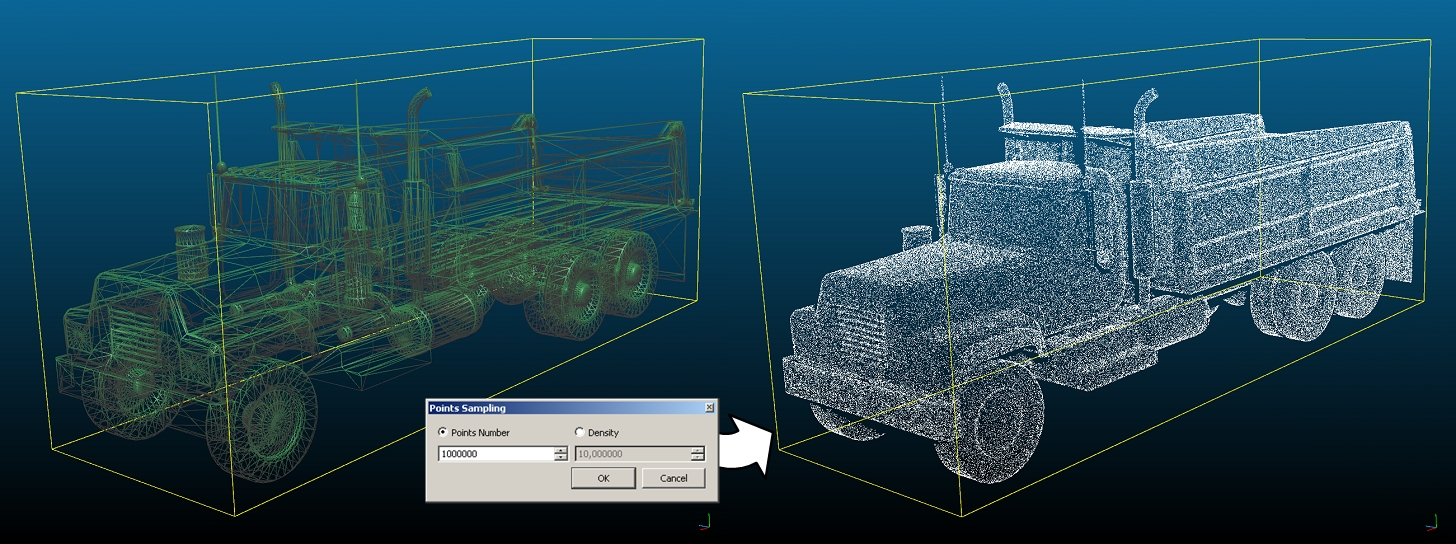
\includegraphics[width=0.9\textwidth]{Partie3_Fonctions/pointsSampling.jpg}
\caption{\label{fig:pointsSampling}Illustration du principe de l'�chantillonnage de points sur un maillage}
\end{center}
\end{figure}

\par
Cette fonction g�n�re un nouveau nuage de points. L'utilisateur � le choix via l'interface~\ref{fig:samplePointsOnMeshDlg} de sp�cifier :
\begin{itemize}
\item soit le nombre total de points d�sir� (approximatif).
\item soit la densit� par unit� de surface. Attention, la surface est exprim�e dans l'unit� implicite (au carr�) des sommets du maillage. Pour conna�tre la surface totale du maillage \index{surface, mesurer}, vous pouvez appeler pr�alablement la fonction << Mesh > Measure surface >> (section~\ref{subsection:measureSurface}).\\
\end{itemize}

\begin{figure}[!h]
\begin{center}
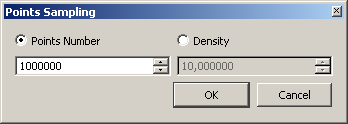
\includegraphics[width=0.3\textwidth]{Partie3_Fonctions/samplePointsOnMeshDlg.png}
\caption{\label{fig:samplePointsOnMeshDlg}Interface pour l'�chantillonnage de points sur un maillage}
\end{center}
\end{figure}

